\chapter{Kịch bản thử nghiệm} \label{chap:experiment}
    \section{Mục tiêu của thử nghiệm}
    \begin{itemize}
        \item Kiểm tra hoạt động của ứng dụng: node gateway thu thập dữ liệu từ các node cảm biến sau đó gửi lên cloud, ấn nút trên node gateway để điều khiển LED trên các node cảm biến.
        \item Chứng minh ứng dụng được hiện thực bằng giao thức mạng Mesh, cụ thể là vai trò của node relay.
        \item Chứng minh các node trong mạng có thể giao tiếp với nhau bằng cả 2 chiều gửi và nhận: node cảm biến gửi dữ liệu cho node gateway và nhận tín hiệu bật/tắt LED từ node gateway.
        \item Kiểm tra khoảng cách hoạt động tối đa giữa các node.
    \end{itemize}
    \section{Quá trình thử nghiệm}
        Nhóm thử nghiệm với 3 board phát triển, một board là node gateway còn lại là node cảm biến lần lượt gọi là node 0 và node 1. Đầu tiên cần tiến hành provision cho 2 node cảm biến: chỉ cần bật nguồn node gateway trước, rồi lần lượt bật nguồn node 0 và node 1. Sau đó tiến hành thử nghiệm bằng các kịch bản sau:
        \subsection{Kịch bản I: Thử nghiệm giao tiếp}
        \begin{itemize}
            \item Đặt 2 node 0 và node 1 ở gần node gateway, sau đó thử ấn nút gửi tín hiệu điều khiển LED thì thấy LED trên cả 2 node cảm biến chớp tắt.
            \begin{figure}[h!]
	    	 \begin{center}
	    		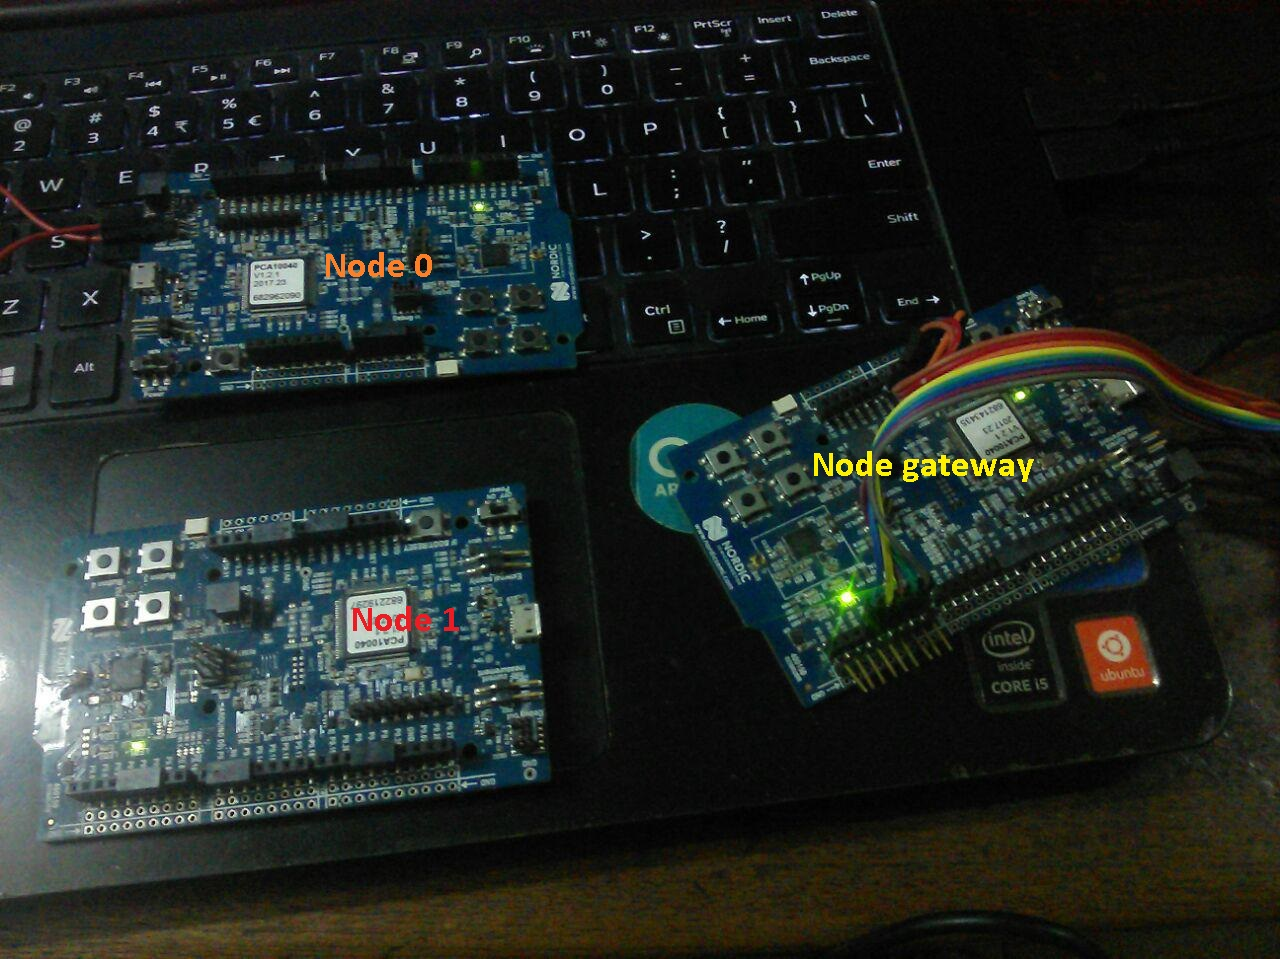
\includegraphics[scale=0.4]{images/ex1-1.jpg}
	    		\caption{Hình ảnh thử nghiệm I trong thực tế}
	    	\end{center}
    	\end{figure}
            \item Sau đó thử kích hoạt chế độ đọc và gửi dữ liệu cảm biến thì thấy node gateway nhận được dữ liệu và gửi lên server thành công. Có thể thử thay đổi dữ liệu bằng cách tăng nhiệt độ ở khu vực gần SoC nRF52832 trên Kit phát triển.
            \begin{figure}[h!]
	    	 \begin{center}
	    		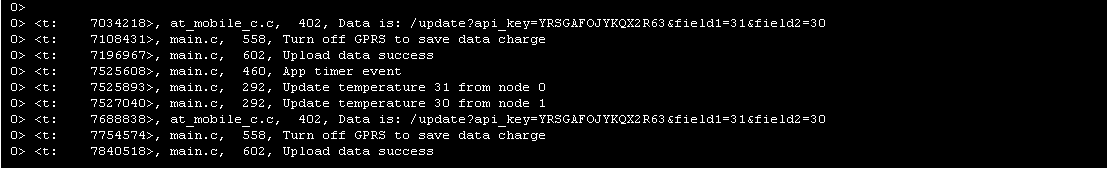
\includegraphics[scale=0.4]{images/ex1-2.png}
	    		\caption{Hình ảnh note gateway nhận được dữ liệu từ node cảm biến}
	    	\end{center}
    	\end{figure}
    	\begin{figure}[h!]
	    	 \begin{center}
	    		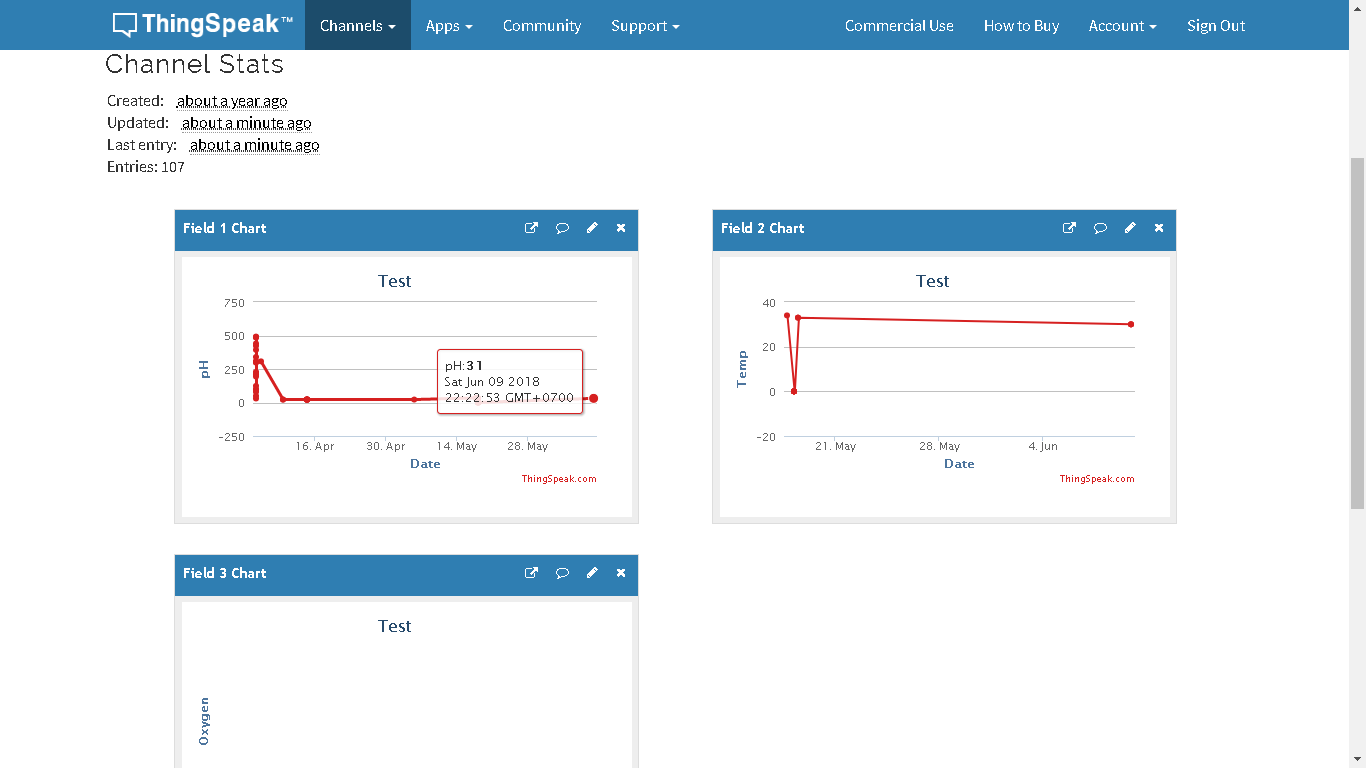
\includegraphics[scale=0.4]{images/ex1-3.png}
	    		\caption{Hình ảnh dữ liệu được cập nhật lên cloud}
	    	\end{center}
    	\end{figure}
            \item Thử tắt nguồn node 0 thì thấy node gateway báo lỗi không đọc được dữ liệu từ node 0, khi bật nguồn lại thì hoạt động bình thường trở lại.
        \end{itemize}
        \textbf{Kết quả thử nghiệm của kịch bản I chứng minh khả năng hoạt động của ứng dụng khi không có lỗi phát sinh.}
        \subsection{Kịch bản II: Thử nghiệm khoảng cách}
        \begin{itemize}
            \item Tiến hành với một node gateway và một node cảm biến là node 0, node gateway sẽ gửi lệnh điều khiển LED liên tục bằng cách nhấn nút.
            \item Sau đó dời node cảm biến dần dần ra xa cho đến khi LED trên node cảm biến không còn chớp tắt nữa thì dừng lại.
            \begin{figure}[h!]
	    	 \begin{center}
	    		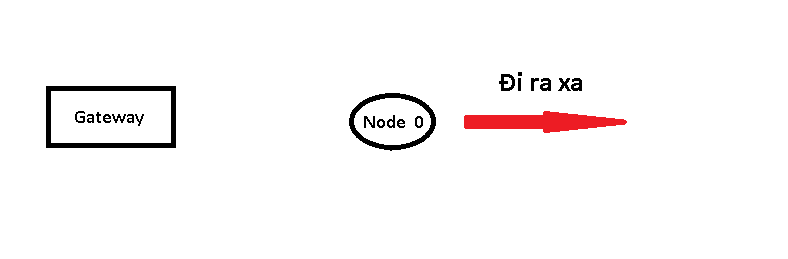
\includegraphics[scale=0.8]{images/ex2-1.png}
	    		\caption{Hình ảnh thử nghiệm II trong thực tế}
	    	\end{center}
        	 \end{figure}
            \item Khoảng cách giữa node gateway và node 0 lúc này là khoảng cách tối đa giữa 2 node của Bluetooth Mesh. Sau đó dời node 0 ra xa thêm khoảng 2m để tiến hành thử kịch bản III.
        \end{itemize}
        \textbf{Kết quả thử nghiệm của kịch bản II chứng tỏ khoảng cách giao tiếp tối đa giữa 2 node trong thực tế (không có vật cản) là khoảng từ 8-10m.}
        \subsection{Kịch bản III: Thử nghiệm truyền dữ liệu trong mạng mesh}
        \begin{figure}[h!]
	    	 \begin{center}
	    		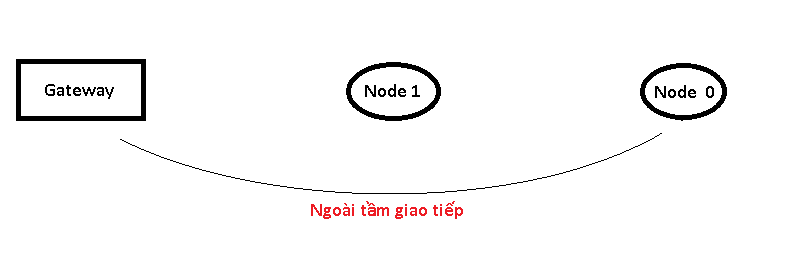
\includegraphics[scale=0.8]{images/ex3-1.png}
	    		\caption{Hình ảnh thử nghiệm III}
	    	\end{center}
        \end{figure}
        \begin{itemize}
            
            \item Sau khi node 0 đã nằm ngoại phạm vi giao tiếp với node gateway, đặt node 1 vào khoảng giữa 2 node này.
            \begin{figure}[h!]
	    	 \begin{center}
	    		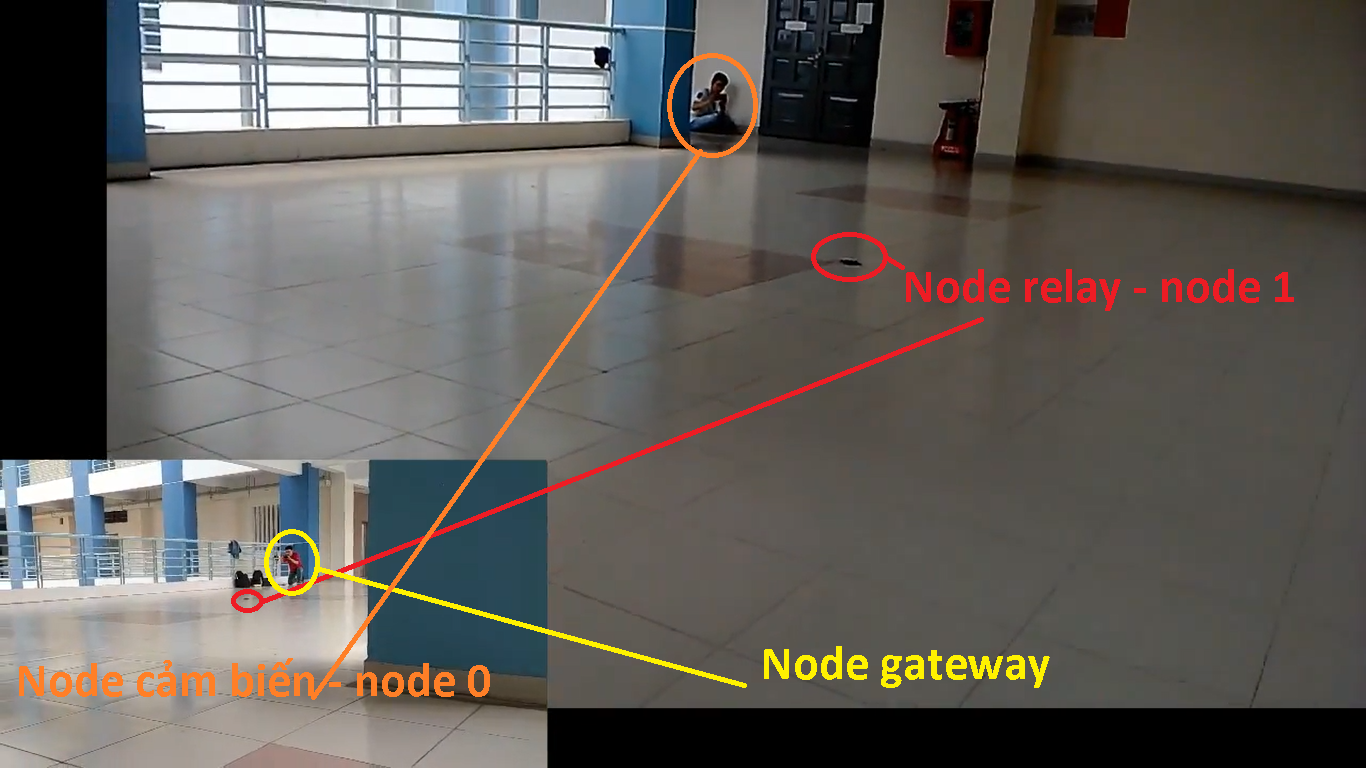
\includegraphics[scale=0.3]{images/ex3-2.png}
	    		\caption{Hình ảnh thử nghiệm III trong thực tế}
	    	\end{center}
    	\end{figure}
    	\newpage
            \item Sau đó tiến hành gửi tín hiệu điều khiển LED bằng node gateway, lúc này LED trên cả node 0 lẫn node 1 đều chớp tắt, chứng tỏ tín hiệu đã được node 1 relay lại và node 0 đã nhận được tín hiệu điều khiển (tín hiệu này gửi multicast nên cả 2 node 0 và 1 đều chớp LED).
            \begin{figure}[h!]
	    	 \begin{center}
	    		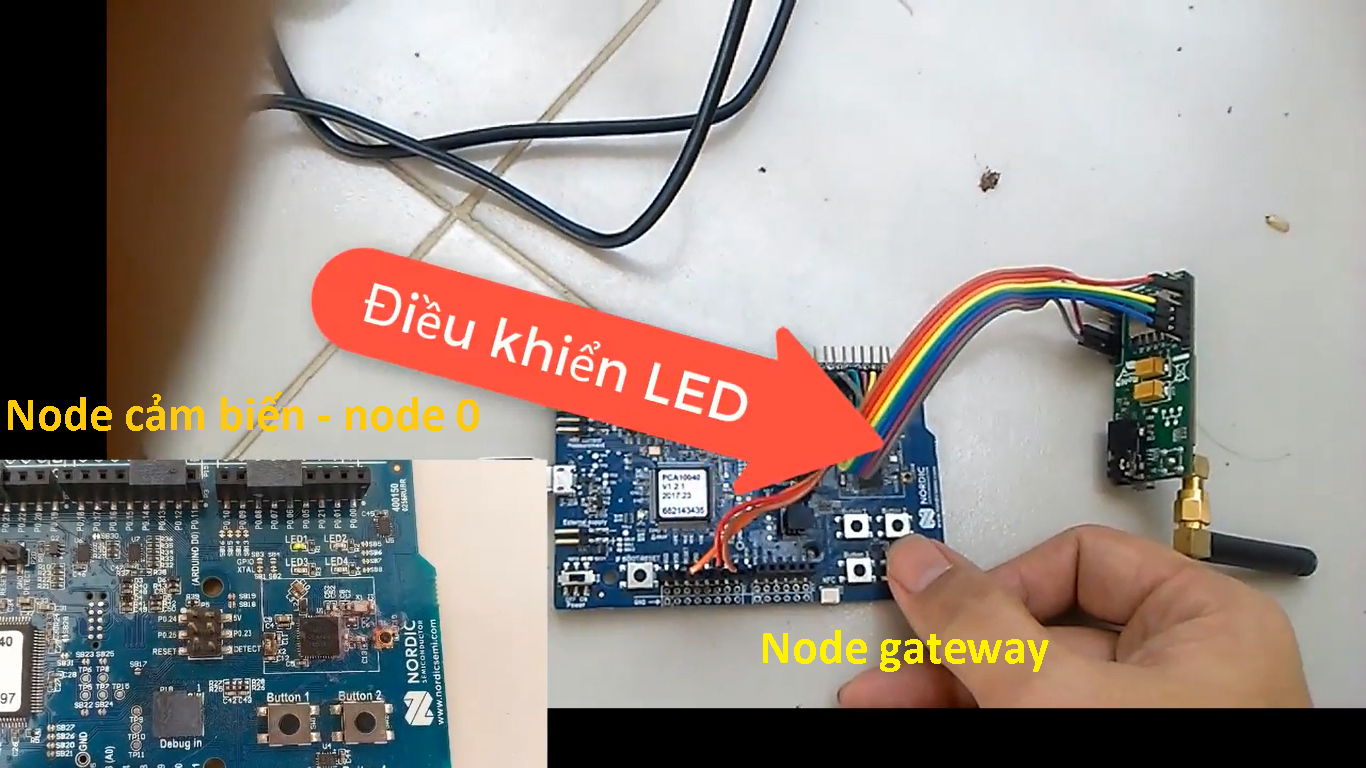
\includegraphics[scale=0.3]{images/ex3-3.png}
	    		\caption{Hình ảnh điều khiển LED trong thực tế}
	    	\end{center}
    	\end{figure}
        \end{itemize}
        \textbf{Kết quả thử nghiệm của kịch bản III chứng tỏ rằng node 1 đã đóng vai trò relay, giúp chuyển tiếp dữ liệu từ node gateway đến cho node 0.}





